% ----------------------------------------------------------------------
% Project:      KalmanApp
% Title:        Summary.tex
% Description:  Details of the algorithm
% 
% --------------------------------------------------------------------
% 
% Copyright (C) 2010-2020 ARM Limited or its affiliates. All rights reserved.
% 
% SPDX-License-Identifier: Apache-2.0
% 
% Licensed under the Apache License, Version 2.0 (the License); you may
% not use this file except in compliance with the License.
% You may obtain a copy of the License at
% 
% www.apache.org/licenses/LICENSE-2.0
% 
% Unless required by applicable law or agreed to in writing, software
% distributed under the License is distributed on an AS IS BASIS, WITHOUT
% WARRANTIES OR CONDITIONS OF ANY KIND, either express or implied.
% See the License for the specific language governing permissions and
% limitations under the License.
% 
\documentclass[titlepage,a4,12pt]{article}
\usepackage{graphics,color}
\usepackage{hyperref}
\usepackage{graphicx}
\usepackage{amsmath}
\usepackage{float}
\usepackage[table]{xcolor}
\usepackage{nccmath}
\usepackage{minted}
\usepackage{lato}


\hypersetup{
colorlinks=true,       % false: boxed links; true: colored links
    linkcolor=red,          % color of internal links (change box color with linkbordercolor)
    citecolor=green,        % color of links to bibliography
    filecolor=magenta,      % color of file links
    urlcolor=cyan,           % color of external links
    pdfauthor={Christophe Favergeon - Copyright (C) 2010-2020 ARM Limited or its affiliates. All rights reserved.},%
    pdftitle={Kalman on Cortex-M with CMSIS-DSP},%
    pagebackref=true
}
\usemintedstyle{monokai}
\definecolor{bg}{rgb}{0,0,0}
\newenvironment{mpmatrix}{\begin{medsize}\begin{pmatrix}}%
{\end{pmatrix}\end{medsize}}%

\numberwithin{equation}{subsection}

\newcommand{\curr}[1]{#1_{k-1|k-1}}
\newcommand{\before}[1]{#1_{k|k-1}}
\newcommand{\after}[1]{#1_{k|k}}

\newcommand{\normal}{n}
\newcommand{\uniform}{u}

\graphicspath{ {./Assets/} }

\title{Kalman on Cortex-M with CMSIS-DSP}
\author{Christophe Favergeon \\ Copyright (C) 2010-2020 ARM Limited or its affiliates.\\ All rights reserved.}
\date{October 2020}
\begin{document}
   \maketitle
\tableofcontents
\newpage
\section{Introduction}
 This document is explaining how to implement an Extended Kalman filter for orientation estimation on a Cortex-M using the CMSIS-DSP library.



\subsection{Kalman filter in a nutshell}

The Kalman filter is the application of a Bayesian filter to a linear  model with normal random variables.

\subsubsection{Linear evolution model}

Let's assume our knowledge of the system is described by a state $\curr{x}$ at instant $k$ and that time is discrete. Let's assume the control is $c_{k}$.

We assume that the new state should be:

\begin{equation} \label{eq:mean}
\before{x} = F\curr{x} + G (c_{k} + n_{k})
\end{equation}

$\before{x}$ is the prediction of the new state at time $k$ based on our knowledge at time $k-1$ which is $\curr{x}$.

It is a prediction because the control is not perfectly known and because a model is always an approximation.

This uncertainty is modeled with a noise $n_k$ which is a centered normal random variable.

As consequence, the state variable must also be a normal variable.

The linear transform of a normal variable is also a normal variable.

So, we just need to compute how the mean and variance are transforming.

The mean is transformed as described with equation \ref{eq:mean}.

If $P$ is the covariance matrix of the normal variable $\curr{x}$ and $Q$ the covariance matrix of the noise $n_k$ then:

\begin{equation} \label{eq:covariance}
\before{P} = F . \curr{P} . F^t + G . Q . G^t
\end{equation}

Note that the noise component was written:

\begin{equation} \label{eq:noisecomponent}
G n_{k}
\end{equation}

Because $n_{k}$ is the noise of a sensor in local coordinates and we can measure it.
The matrix $G$ is doing a conversion to world coordinate.


\subsubsection{Observation}

The covariance matrix of the state variable has been changed by the evolution. We are less certain about the state.

We want to update our knowledge about the state from the observation.

We want to compute:

\begin{equation} 
p(\after{x} | z_k)
\end{equation}

where $z_k$ is the observation and $\after{x}$ is our knowledge of the state for time $k$ based on the evolution model ($\before{x}$) and the observation.

Using Bayes theorem, we can compute this as:

\begin{equation} 
p(x | z_k) = \frac{p(z_k | \before{x}) p(\before{x})}{p(z_k)}
\end{equation}


$p(z_k | \before{x})$ is given by the observation model which is assumed to be linear.

\begin{equation} 
z_k = H . \before{x} + r_k
\end{equation}

where $r_k$ is the observation noise with covariance matrice $R$ (and assumed to have a zero mean).

$p(\after{x} | z_k)$ is a normal variable so we need to compute its mean and covariance matrix. The most likely value will be the mean.

After some computations which are a bit tricky, we finally get the update equations:

\begin{align}
y_k &= z_k - H . \before{x} \\
S_k &= H . \before{P} . H^t + R \\ 
K &= \before{P} . H^t . S_k^{-1} \\ 
\after{x} &= \before{x} + K . y_k \\ 
\after{P} &= (I - K . H) \before{P}
\end{align}

And this is the Kalman filter.

\subsection{Quaternion}

Orientation will be described using a normalized quaternion.

A normalized quaternion $(q_0,q_1,q_2,q_3)$ is corresponding to the following rotation matrix:

\begin{equation}\label{eq:quattorot}
R = \left(
\begin{array}{ccc}
 q_0^2+q_1^2-q_2^2-q_3^2 & 2 (q_1 q_2-q_0 q_3) & 2 (q_0 q_2+q_1 q_3) \\
 2 (q_0 q_3+q_1 q_2) & q_0^2-q_1^2+q_2^2-q_3^2 & 2 (q_2 q_3-q_0 q_1) \\
 2 (q_1 q_3-q_0 q_2) & 2 (q_0 q_1+q_2 q_3) & q_0^2-q_1^2-q_2^2+q_3^2 \\
\end{array}
\right)
\end{equation}

This matrix $R$ is describing the transformation to apply to the body to get its position in space.

As a consequence, a vector $\overrightarrow{v}$ measured in the body coordinate is corresponding to a vector $R^t . \overrightarrow{v}$ in world coordinates since $R^t$ is the inverse of $R$.

The body is rotating. To know how the quaternion is transformed due to this rotation in an infinitesimal duration, we need to use the angular speed $(\omega_x, \omega_y, \omega_z)$ and compute the following matrix:

\begin{equation}\label{eq:quatrot}
S(\omega) = \left(
\begin{array}{cccc}
 0 & -\omega_x & -\omega_y & -\omega_z \\
 {\omega_x} & 0 & {\omega_z} & -{\omega_y} \\
 {\omega_y} & -{\omega_z} & 0 & {\omega_x} \\
 {\omega_z} & {\omega_y} & -{\omega_x} & 0 \\
\end{array}
\right)
\end{equation}

The derivative of the quaternion $q$ is given by :

\begin{equation}
q' = \frac{1}{2} S(\omega) q
\end{equation}

So, we can write the update equation of the quaternion as:

\begin{align} \label{eq:update}
q_0(t+dt) = q_0 + \frac{1}{2} \text{dt} (-q_1 \omega_x-q_2 \omega_y-q_3 \omega_z)\\
q_1(t+dt) = q_1 + \frac{1}{2} \text{dt} (q_0 \omega_x+q_2 \omega_z-q_3 \omega_y)\\
q_2(t+dt) = q_2 + \frac{1}{2} \text{dt} (q_0 \omega_y-q_1 \omega_z+q_3 \omega_x)\\
q_3(t+dt) = q_3 + \frac{1}{2} \text{dt} (q_0 \omega_z+q_1 \omega_y-q_2 \omega_x)
\end{align}

This update equation is corresponding to the Euler integration scheme.
It is not the most accurate and a Runge–Kutta method may be preferred. 

Note that the speed $\omega$ is expressed in local coordinates. The rotation of the body is in world coordinates. The equation \ref{eq:update} is taking this into account.


\section{Prediction}

With quaternions, the update equations are no more linear.
So, to be able to apply the Kalman update formula, we linearise the equations around the current point : it is the extended Kalman filter.

The evolution model is a non linear function $f$.

The matrixes to be applied to the state covariance and process covariances are $F_k$ and $G_k$ and must be recomputed at each time step. They are extracted from the Jacobian matrix of $f$. $F_k$ is the part related to state variables and $G_k$ is the part related to control variables. In the code $G$ is also named $FQ$. 

The new update equation is very similar to the ones in \ref{eq:mean} and \ref{eq:covariance}.

For the update of the mean, $f$ is used instead of the $F$ matrix.

For the update of the covariance, we use the new matrixes $F_k$ and $G_k$.

$F$ is related to the state variables and $G$ to the control ones.

\begin{align}\label{eq:predict}
\before{x} &= f(\curr{x},c_k)\\
\before{P} &= F_k . \curr{P} . F_k^t + G_k . Q . G_k^t
\end{align}

$Q$ is the covariance matrix of the control variables.

The formula for $f$ is just giving the quaternion update for a given duration $dt$.

It is important to note that the covariance noise due to control has to be updated each time since it depends on the matrix $G_k$.

For the linear filter, $G_k$ being constant, the noise convariance is fixed. It is not the case here.

$c_k$ is $\omega_k$ since the control is the angular speed measured by the gyro. Starting from now, we will note $\omega$ with $w$ to be closer to the final C code.

\begin{equation}\label{eq:f}
f = \left(
\begin{array}{c}
 \frac{1}{2} \text{dt} (-q_1 {w_x}-q_2 {w_y}-q_3 {w_z})+q_0 \\
 \frac{1}{2} \text{dt} (q_0 {w_x}+q_2 {w_z}-q_3 {w_y})+q_1 \\
 \frac{1}{2} \text{dt} (q_0 {w_y}-q_1 {w_z}+q_3 {w_x})+q_2 \\
 \frac{1}{2} \text{dt} (q_0 {w_z}+q_1 {w_y}-q_2 {w_x})+q_3 \\
\end{array}
\right)
\end{equation}

The derivative according to the state and control variables are giving by the matrixes:

\begin{equation}\label{eq:Fmatrix}
F_k = \left(
\begin{array}{cccc}
 1 & -\frac{\text{dt} {w_x}}{2} & -\frac{\text{dt} {w_y}}{2} & -\frac{\text{dt} {w_z}}{2} \\
 \frac{\text{dt} {w_x}}{2} & 1 & \frac{\text{dt} {w_z}}{2} & -\frac{\text{dt} {w_y}}{2} \\
 \frac{\text{dt} {w_y}}{2} & -\frac{\text{dt} {w_z}}{2} & 1 & \frac{\text{dt} {w_x}}{2} \\
 \frac{\text{dt} {w_z}}{2} & \frac{\text{dt} {w_y}}{2} & -\frac{\text{dt} {w_x}}{2} & 1 \\
\end{array}
\right)
\end{equation}

\begin{equation}\label{eq:Gmatrix}
G_k = FQ_k =\left(
\begin{array}{ccc}
 -\frac{\text{dt} q_1}{2} & -\frac{\text{dt} q_2}{2} & -\frac{\text{dt} q_3}{2} \\
 \frac{\text{dt} q_0}{2} & -\frac{\text{dt} q_3}{2} & \frac{\text{dt} q_2}{2} \\
 \frac{\text{dt} q_3}{2} & \frac{\text{dt} q_0}{2} & -\frac{\text{dt} q_1}{2} \\
 -\frac{\text{dt} q_2}{2} & \frac{\text{dt} q_1}{2} & \frac{\text{dt} q_0}{2} \\
\end{array}
\right)
\end{equation}

\section{Observation}

The observation update equations are nearly the same but since the observation is not linear, we need to use a non linear function $h$ to update the mean and the Jacobian matrix $H_k$ to update the covariance.

The formula is thus:

\begin{align}\label{eq:observe}
y_k &= z_k - h(\before{x})\\
S_k &= H_k . \before{P} . H_k^t + R_k\\
Ka_k&= \before{P} . H_k^t . S^{-1}_k \\
\after{x} &= \before{x} + Ka_k . y_k \\ 
\after{P} &= (I - Ka_k . H_k) . \before{P}
\end{align}

The rotation matrix $R$ to apply to the body to get its orientation is allowing us to convert a vector from the world frame to the body frame using $R^t$.
(In the equation \ref{eq:observe}, $R_k$ is not the rotation but the observation noise covariance. This naming is to be coherent with the source code of the implementation.)


So, when we express the body acceleration $\overrightarrow{acc_{body}}$ we should have:

\begin{equation}\label{eq:accworld}
\overrightarrow{acc_{body}} = R^t . \left(
\begin{array}{c}
 0 \\
 0 \\
 -9.815 \\
\end{array}
\right)
\end{equation}

Similarly, when we express the body magnetic field in the world frame we should get:

\begin{equation}\label{eq:magworld}
\overrightarrow{mag_{body}} = R^t . \left(
\begin{array}{c}
 -1 \\
 0 \\
 0 \\
\end{array}
\right)
\end{equation}

So our $x$ axis in the world frame of reference is from north to south.

And we get the observation function $h$ :

\begin{equation}\label{eq:h}
h = \left(
\begin{array}{c}
 -19.62 (q_1 q_3-q_0 q_2) \\
 -19.62 (q_0 q_1+q_2 q_3) \\
 -9.81 \left(q_0^2-q_1^2-q_2^2+q_3^2\right) \\
 -1. \left(q_0^2+q_1^2-q_2^2-q_3^2\right) \\
 -2. (q_1 q_2-q_0 q_3) \\
 -2. (q_0 q_2+q_1 q_3) \\
\end{array}
\right)
\end{equation}

And the linearized $H_k$ is given by:

\begin{equation}\label{eq:Hmatrix}
H_k=\begin{mpmatrix}
 19.62 q_2 & -19.62 q_3 & 19.62 q_0 & -19.62 q_1 \\
 -19.62 q_1 & -19.62 q_0 & -19.62 q_3 & -19.62 q_2 \\
 -19.62 q_0 & 19.62 q_1 & 19.62 q_2 & -19.62 q_3 \\
 -2. q_0 & -2. q_1 & 2. q_2 & 2. q_3 \\
 2. q_3 & -2. q_2 & -2. q_1 & 2. q_0 \\
 -2. q_2 & -2. q_3 & -2. q_0 & -2. q_1 \\
\end{mpmatrix}
\end{equation}

If the orientation estimation is wrong then the observation will be different from the expected gravity and magnetic field.

Note that during a movement, the board will measure the gravity and acceleration of the board.

So the gravity reference will be lost and this update equation will no more be useful. It is only when the board is kept still (or not moving too quicky) that this will allow the Kalman filter to converge and estimate some orientation.


\section{Sensors and calibration}

Observation equations are requiring the noise covariance $R$ and the evolution equations are requiring the control noise $Q$.

It has to be measured. A normal distribution should be fitted to the noise.


\subsection{Magnetometer}

The magnetometer needs to be calibrated.

We expect the measurements to be on a sphere. They generally will be on an ellipse.

We expect the sphere to be centered in $(0,0,0)$ and it won't be the case.

Finally, since we are only interested in the direction of the magnetic field, we expect the sphere to have a radius of $1$.

Here in blue we have the target sphere and in red the measured one.

\begin{figure}[H]
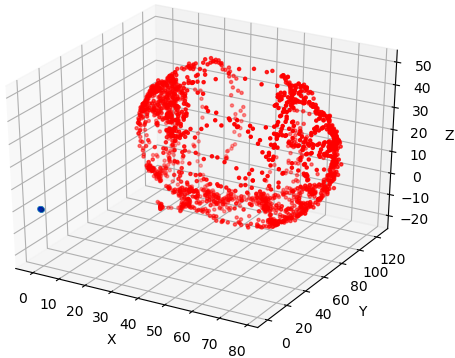
\includegraphics{uncalibratedmag.png}
\end{figure}

After calibration, the red dots are on the blue sphere.

\begin{figure}[H]
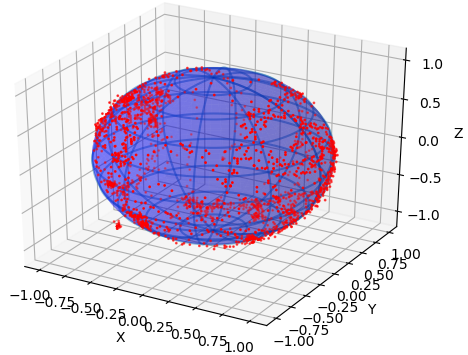
\includegraphics{calibratedmag.png}
\end{figure}

To do this calibration, we need to apply an offset and a matrix.
\begin{equation}
\overrightarrow{CM_{body}} = M.  (\overrightarrow{M_{body}} - \overrightarrow{offset})
\end{equation}

$\overrightarrow{CM_{body}}$ is the calibrated measurement.


To fit an ellipse to a cloud of point, the following article was used:
\url{https://ieeexplore.ieee.org/document/1290055}

To map the ellipse onto a unit sphere, the following article was used:
\url{https://ieeexplore.ieee.org/document/6289882}

\subsection{Gyroscope}

According to the litteratue, it looks like the biases in the gyroscope noise are real and not just a measurement error.

Since the angular speeds are integrated, those biases will result in a drift.
So the orientation estimation will diverge.

Those biases should be removed from the measurement before integrating.

But we can expect those biases to evolve in time (dependence on temperature etc ...). There is no automatic way (from this Kalman) to estimate those biases again. There are not enough observations and too many degree of freedom if the biases are included in the state vector.

Those biases would have to be measured again from time to time.

\section{Implementation}
\subsection{Prediction}

A macro is used to access the matrix elements using a (row,column) specification.

\begin{minted}[bgcolor=bg]{c}
#define M(A,r,c) (A.pData[r * A.numCols + c])
\end{minted}

We update the quaternion using the equation \ref{eq:f}.
Then we normalize the quaternion because only a normalized quaternion is representing a rotation and we want to prevent rounding errors from breaking this property.

\begin{minted}[bgcolor=bg]{c}
f_update();

normalizeQuat(&NQ0,&NQ1,&NQ2,&NQ3);
\end{minted}

Then, the $F_k$ and $G_k$ matrixes are computed using equations \ref{eq:Fmatrix}
and \ref{eq:Gmatrix}

The code is generated from a computer algebra system since it is the part of the implementation to be changed each time the model is changed.

As consequence, this code is not optimized. A better generation procedure could take into account the symmetry of the matrixes and the possibility of vectorizing to generate a better code.

\begin{minted}[bgcolor=bg]{c}
F_update();

FQ_update();
\end{minted}

We update covariance using equation \ref{eq:predict}.

$OmegaErrors$ is the covariance matrix for the gyro errors (in the equation it is named $Q$). Here, in the code, $Q$ is the result after applying the $G_k$ matrix.

We symmetrize the covariance matrix $NP$ by copying the upper triangle onto the lower one. It is to ensure that, in spite of rounding errors, the matrix is still symetric and definite positive.

$NP$ is $\before{P}$.

\begin{minted}[bgcolor=bg]{c}
// Update covariance
arm_mat_mult_f32(&F,&P,&Temp1_NS_NS);
arm_mat_trans_f32(&F,&Temp2_NS_NS);
arm_mat_mult_f32(&Temp1_NS_NS,&Temp2_NS_NS,&Temp3_NS_NS);
  
arm_mat_mult_f32(&G,&OmegaErrors,&Temp1_NS_NC);
arm_mat_trans_f32(&G,&Temp2_NC_NS);
arm_mat_mult_f32(&Temp1_NS_NC,&Temp2_NC_NS,&Q);
  
arm_mat_add_f32(&Temp3_NS_NS,&Q,&NP);
symmetrize(&NP);

\end{minted}

\subsection{Observation}

The observation is computed following \ref{eq:h}

We predict the acceleration and magnetic field in the body frame.

\begin{minted}[bgcolor=bg]{c}
h_update();
\end{minted}

The $H$ matrix is computed following equation \ref{eq:Hmatrix}.

The code is generated from a computer algebra system.

\begin{minted}[bgcolor=bg]{c}
H_update();
\end{minted}

Then we apply the observation step of the Kalman filter following equations \ref{eq:observe}

First, the Kalman gain is computed.

\begin{minted}[bgcolor=bg]{c}
arm_sub_f32(obs,predictedobs,y,NBOBS);


// Compute S
// (obs , state) x (state,state) -> (obs, state) 
// H . P{k|k-1}
arm_mat_mult_f32(&H,&NP,&Temp4_NO_NS);
// (obs,state) -> (state,obs)
arm_mat_trans_f32(&H,&Temp5_NS_NO);
// (obs,state) x (state,obs) -> (obs,obs)
// H . P{k|k-1} . H^t
arm_mat_mult_f32(&Temp4_NO_NS,&Temp5_NS_NO,&Temp6_NO_NO);
// H . P{k|k-1} . H^t + R
arm_mat_add_f32(&Temp6_NO_NO,&R,&S);
   

// Compute K 
// (state,state) x (state,obs) -> (state,obs)
// P{k|k-1} . H^t
arm_mat_mult_f32(&NP,&Temp5_NS_NO,&Temp7_NS_NO);

arm_mat_inverse_f32(&S,&Temp8_NO_NO);

// (state,obs) x (obs,obs) -> (state,obs)
// P{k|k-1} . H^t . S^-1
arm_mat_mult_f32(&Temp7_NS_NO,&Temp8_NO_NO,&K);
\end{minted}

The matrix inversion should use the Cholesky algorithm. But it is not (yet) available in CMSIS-DSP.
So, the standard Gauss-Jordan algorithm is used. It is not the right way but it is enough for this demo where the simulation is running for a limited number of samples.


The Kalman gain is used to update the state and covariance matrix of the state.

\begin{minted}[bgcolor=bg]{c}
// Equation 3.0.4

arm_mat_vec_mult_f32(&K,y,oldstate);
// x{k|k-1}  + K y
arm_add_f32(oldstate,newstate,oldstate,NBSTATE);



// Update covariance
// Equation 3.0.5
arm_mat_mult_f32(&K, &H,&Temp1_NS_NS);
arm_mat_sub_f32(&Identity_NS_NS,&Temp1_NS_NS,&Temp2_NS_NS);
arm_mat_mult_f32(&Temp2_NS_NS,&NP,&P);

symmetrize(&P);
\end{minted}

The version $1.9.0$ of the CMSIS-DSP must be used otherwise the function $arm\_mat\_vec\_mult\_f32$ won't be available.


\subsection{Limitations}

\subsubsection{Matrix inversion}

It is a critical part of the algorithm. Current solution (Gauss-Jordan) is not the right way.
As soon as Cholesky is added to the CMSIS-DSP, this demo will be updated to use it.

\subsubsection{Update}

We update the Kalman filter as quickly as possible to ensure that the duration $dt$ used for the integration (in the prediction step) is as low as possible.

But the sensors are not refreshing as often. So, we reuse the last measured value when no new value is available.


Different strategies need to be tested : updating only when a new measurement is available and thus accepting to use bigger $dt$ when integrating the angular speed.

Using a low pass filtered version of the sensor values instead of reusing the last measurements (interpolation of the values).

Or with playing with the covariance matrices of the noise : increasing the coefficient related to a specific sensor when no new data is available for this sensor. By doing this, the filter will give less importance to the reused sample.

\section{Conclusions}

Tuning an extended Kalman filter is difficult. There are several parameters (covariance matrix of noises) which can be modified. The right trade-off is not easy to find.

The sensors need to be calibrated which is not easy.

Some sensors may have defect (biases) which are evolving in time and it should be taken into account.

In summary : This is a proof of concept. More work is required to get a real implementation from this code.

\end{document}